\section{Условие}

{\bfseries Цель работы:} \\
Приобретение практических навыков в:
\begin{itemize}
\item Управление процессами в ОС
\item Обеспечение обмена данных между процессами посредством каналов
\end{itemize}

{\bfseries Задание:} \\
Составить и отладить программу на языке Си, осуществляющую работу с процессами и
взаимодействие между ними в одной из двух операционных систем. В результате работы
программа (основной процесс) должен создать для решение задачи один или несколько
дочерних процессов. Взаимодействие между процессами осуществляется через системные
сигналы/события и/или каналы (pipe).
Необходимо обрабатывать системные ошибки, которые могут возникнуть в результате работы.

\begin{figure}[h]
    \centering
    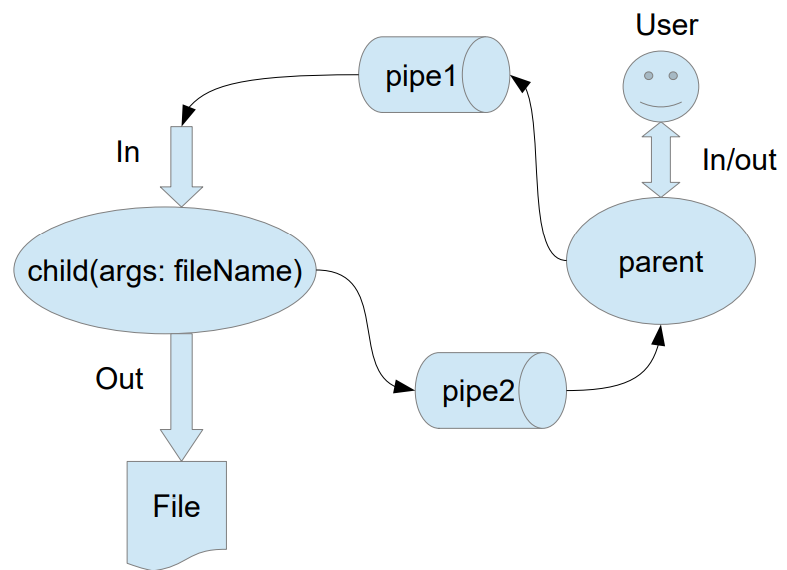
\includegraphics[width=0.75\textwidth]{src/shema.png}
    \caption{Схема работы процессов.}
    \label{fig:schema}
\end{figure}

{\bfseries Вариант:} 4 \\
Родительский процесс создает дочерний процесс. Первой строчкой пользователь в консоль
родительского процесса пишет имя файла, которое будет передано при создании дочернего
процесса. Родительский и дочерний процесс должны быть представлены разными программами.
Родительский процесс передает команды пользователя через pipe1, который связан с
стандартным входным потоком дочернего процесса. Дочерний процесс принеобходимости
передает данные в родительский процесс через pipe2. Результаты своей работы дочерний
процесс пишет в созданный им файл. Допускается просто открыть файл и писать туда, не
перенаправляя стандартный поток вывода.
Пользователь вводит команды вида: «число число число<endline>». Далее эти числа
передаются от родительского процесса в дочерний. Дочерний процесс производит деление первого числа, на последующие, а результат выводит в файл. Если происходит деление на 0, то
тогда дочерний и родительский процесс завершают свою работу. Проверка деления на 0 должна
осуществляться на стороне дочернего процесса. Числа имеют тип float. Количество чисел может
быть произвольным.